\documentclass[11pt,letterpaper]{article}

% ---------- Paquetes ----------
\usepackage[utf8]{inputenc}
\usepackage[T1]{fontenc}
\usepackage[margin=2.5cm]{geometry}
\usepackage{tikz}
\usepackage{graphicx}
\usetikzlibrary{shapes.multipart, arrows.meta, positioning}
\usepackage{forest}
\usepackage{titlesec}
\usepackage{enumitem}
\usepackage{xcolor}
\usepackage{hyperref}
\usepackage{fontawesome5}
\hypersetup{colorlinks=true, linkcolor=black, urlcolor=blue}

% ---------- Formato de títulos ----------
\titleformat{\section}{\large\bfseries}{\thesection.}{0.5em}{}
\titleformat{\subsection}{\normalsize\bfseries}{\thesubsection.}{0.5em}{}

\title{\vspace{-1.5cm}\textbf{Automatización de Horarios y Turnos}\\[0.3em]
\large Entrega 1 -- Definición del Proyecto}
\author{}
\date{}

\begin{document}

% ================= PORTADA =================
\begin{titlepage}
    \centering
    \vspace*{1cm}
    {\Large\bfseries Universidad Andrés Bello}\\[0.2cm]
    {\large Facultad de Ingeniería -- Escuela de Computación e Informática}\\[0.2cm]
    {\large Ingeniería de Software I -- PTEC105}\\[2cm]

    {\Huge\bfseries Automatización de Horarios y Turnos}\\[0.5cm]
    {\Large Entrega 1: Contexto, Problemática, Solución, EDT e Ishikawa}\\[2.5cm]

    \begin{minipage}{0.85\textwidth}
        \centering
        \large\bfseries Integrantes
        \vspace{0.5cm}

        \begin{tabular}{l l}
            \textbf{Benjamin Candia}  & \\[-0.1cm]
            \small Correo institucional: \href{mailto:b.candiagarrido@undresbello.edu}{b.candiagarrido@undresbello.edu} & \\[0.4cm]

            \textbf{Ignacio Figueroa} & \\[-0.1cm]
            \small Correo institucional: \href{mailto:i.figueroacontreras@undresbello.edu}{i.figueroacontreras@undresbello.edu} &  \\[0.4cm]

            \textbf{Endert Guerrero}  & \\[-0.1cm]
            \small Correo institucional: \href{mailto:e.guerrerocamacho@undresbello.edu}{e.guerrerocamacho@undresbello.edu} &  \\[0.4cm]

            \textbf{Felipe Ochoa}     & \\[-0.1cm]
            \small Correo institucional: \href{mailto:f.ochoajohn@uandresbello.edu}{f.ochoajohn@uandresbello.edu}   \\[0.4cm]

            \textbf{Jorge Pinto}      & \\[-0.1cm]
            \small Correo institucional: \href{mailto:j.pintogomez@undresbello.edu}{j.pintogomez@undresbello.edu} &  \\[0.4cm]

            \textbf{Antonia Valdebenito}      & \\[-0.1cm]
            \small Correo institucional: \href{mailto:a.valdebenitofuentes@undresbello.edu}{a.valdebenitofuentes@undresbello.edu} &  \\[0.4cm]
        \end{tabular}
    \end{minipage}

    \vfill

    \begin{tabular}{ll}
        \textbf{Profesor:} & Álvaro Sánchez Colmenares \\[0.2cm]
        \textbf{Fecha de entrega:} & 23 de agosto de 2026 \\
    \end{tabular}

    \vspace{1cm}
\end{titlepage}

\tableofcontents
\newpage

% ================= CONTEXTO =================
\section{Contexto}

Muchas organizaciones con personal por turnos (retail, clínicas, \textit{call centers}, restaurantes) todavía arman sus horarios de forma manual, utilizando planillas de cálculo o incluso papel. Un jefe de turno o encargado de Recursos Humanos debe cruzar manualmente la disponibilidad de cada trabajador, las horas mínimas y máximas permitidas por ley, los días de descanso obligatorios y las necesidades de cobertura por horario. Este proceso se repite semana a semana y, a medida que el equipo de trabajo crece, se vuelve cada vez más difícil de sostener sin errores.

% ================= PROBLEMÁTICA =================
\section{Problemática}

A partir del contexto anterior, se identifican los siguientes problemas recurrentes:

\begin{itemize}[leftmargin=1.2cm]
    \item \textbf{Errores humanos frecuentes}: choques de turno (dos personas asignadas al mismo horario crítico, o ningún trabajador asignado), o turnos que no respetan el descanso mínimo legal entre jornadas.
    \item \textbf{Tiempo perdido}: armar el horario semanal puede tomar horas, y cualquier cambio de última hora (una licencia médica, una renuncia) obliga a rehacer todo manualmente.
    \item \textbf{Falta de trazabilidad}: los cambios y canjes de turno se coordinan verbalmente o por aplicaciones de mensajería, sin quedar registrados en ningún sistema.
    \item \textbf{Comunicación tardía}: los horarios se publican con poca anticipación, generando reclamos y ausentismo.
    \item \textbf{Sobrecarga desigual}: sin una vista centralizada, es común que algunos trabajadores terminen con muchas más horas que otros.
\end{itemize}

% ================= SOLUCIÓN =================
\section{Posible Solución}

Se propone el desarrollo de un sistema de software que automatice la generación y gestión de turnos de trabajo, considerando las siguientes capacidades principales:

\begin{itemize}[leftmargin=1.2cm]
    \item Registro de disponibilidad, roles y restricciones legales de cada trabajador.
    \item Generación automática de una propuesta de horario semanal o mensual, respetando reglas de negocio (cobertura mínima, descansos obligatorios, horas máximas).
    \item Gestión de solicitudes de cambio o canje de turno entre trabajadores, con aprobación del encargado.
    \item Notificación automática del horario publicado y de cualquier modificación posterior.
    \item Historial trazable de asignaciones, cambios y aprobaciones.
\end{itemize}

\subsection{Alcance funcional (módulos del sistema)}

El sistema se organiza en cinco módulos principales:

\begin{itemize}[leftmargin=1.2cm]
    \item \textbf{Gestión de usuarios}: creación de cuentas, roles y permisos (administrador, jefe de turno, trabajador), autenticación y control de acceso.
    \item \textbf{Gestión de trabajadores}: ficha de cada trabajador con datos personales, rol, disponibilidad, restricciones y contrato laboral.
    \item \textbf{Gestión de horarios}: generación, publicación y edición de turnos, solicitudes de cambio/canje y su aprobación.
    \item \textbf{Cumplimiento de la jornada laboral}: validación automática de descansos mínimos, horas máximas diarias/semanales y alertas de incumplimiento según normativa vigente.
    \item \textbf{Reportería estadística}: reportes de horas trabajadas, ausentismo, cumplimiento normativo y carga de trabajo por trabajador/periodo.
\end{itemize}

% ================= EDT =================
\section{Estructura de Desglose del Trabajo (EDT)}

La Figura~\ref{fig:edt} presenta la EDT del proyecto, organizada en cinco fases principales, alineadas con las unidades del curso. Cada fase ha sido desglosada en sus entregables clave para asegurar el cumplimiento de los objetivos.
\begin{figure}[h!]
\centering
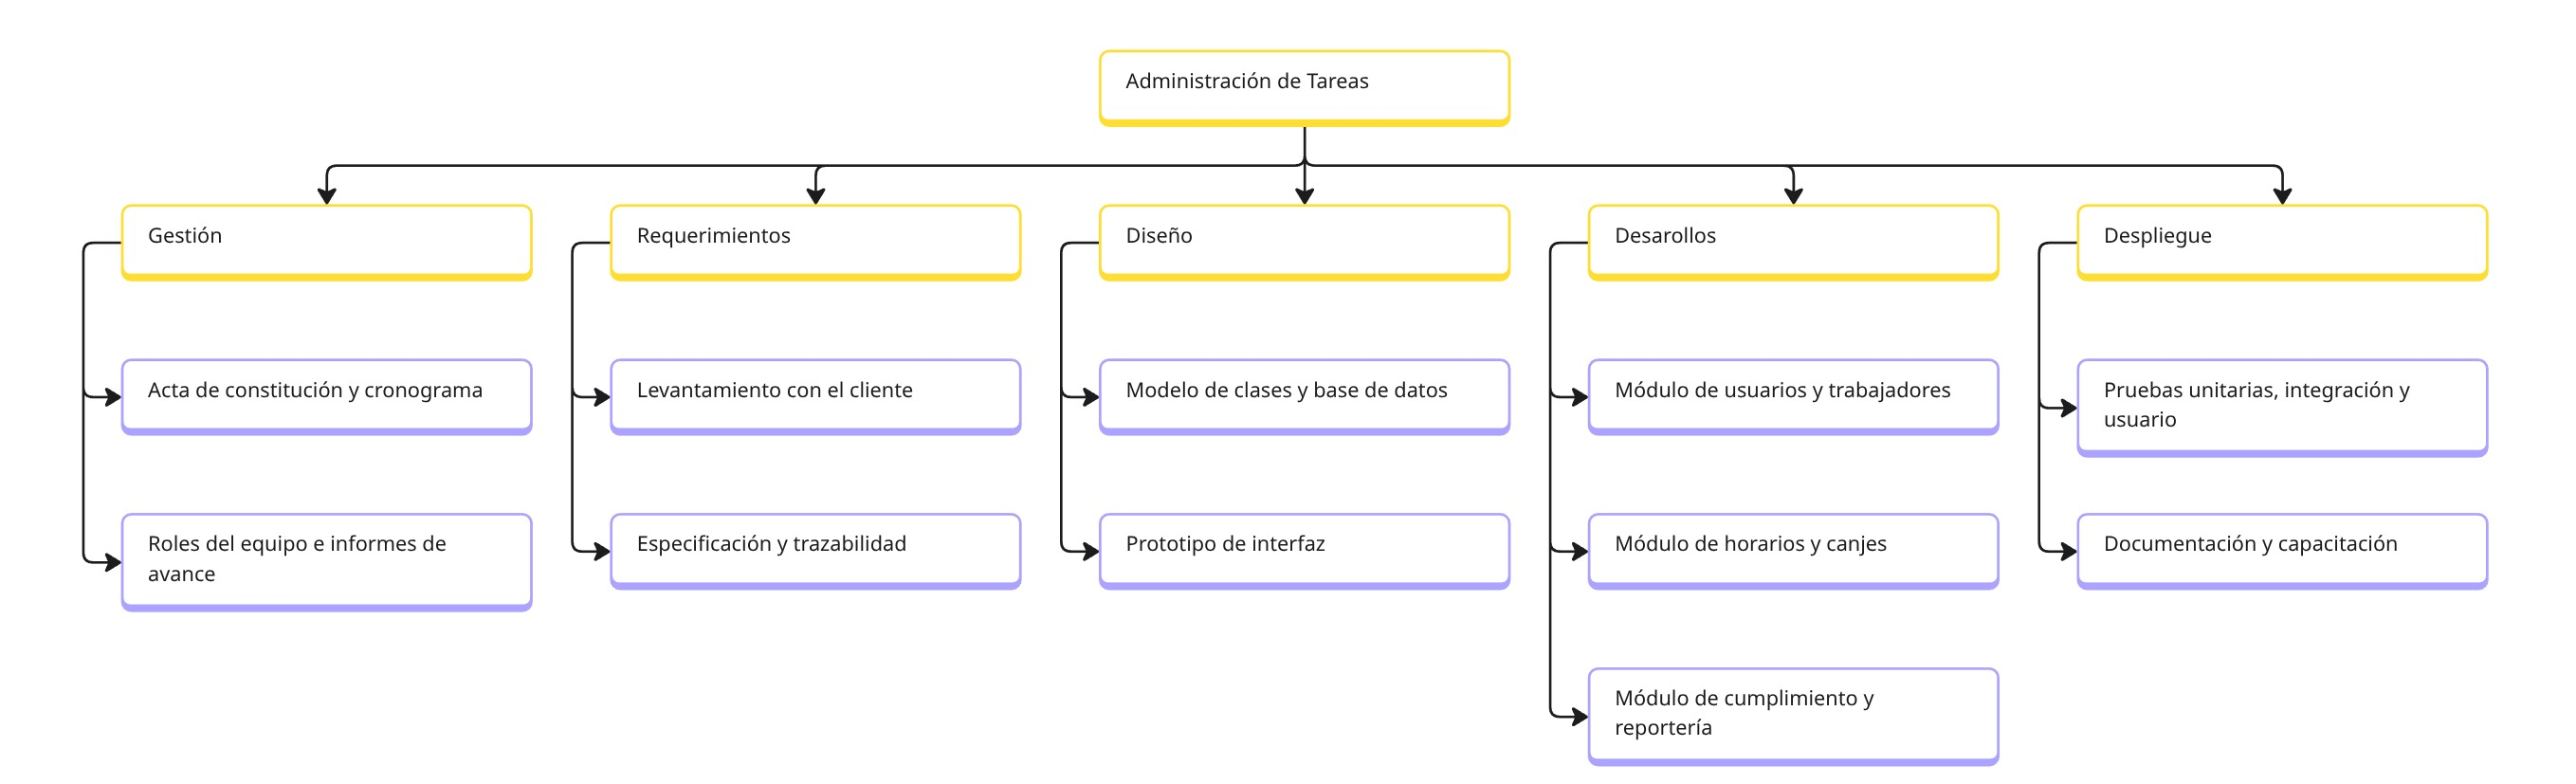
\includegraphics[width=0.9\textwidth]{Estructura de desglose de trabajo.jpg}
\caption{Estructura de Desglose del Trabajo (EDT) del proyecto.}
\label{fig:edt}
\end{figure}

\noindent Cada fase se descompone en los siguientes entregables:

\begin{itemize}[leftmargin=1.2cm]
    \item \textbf{Gestión}: acta de constitución, cronograma, roles del equipo, informes de avance semanales.
    \item \textbf{Requisitos}: entrevistas con el cliente, requisitos funcionales y no funcionales, historias de usuario, trazabilidad.
    \item \textbf{Diseño}: modelo de clases, diagrama de base de datos, prototipo de interfaz, patrones de diseño a utilizar.
    \item \textbf{Desarrollo}: módulo de gestión de usuarios, módulo de gestión de trabajadores, módulo de gestión de horarios (motor de asignación automática y canjes/aprobaciones), módulo de cumplimiento de la jornada laboral y módulo de reportería estadística.
    \item \textbf{Despliegue}: pruebas unitarias e integración, pruebas de usuario, documentación y capacitación.
\end{itemize}

% ================= ISHIKAWA =================
\section{Diagrama de Ishikawa (Causa-Efecto)}

La Figura~\ref{fig:ishikawa} presenta el diagrama de Ishikawa que resume las causas raíz de los errores y demoras en la asignación manual de turnos. Se han identificado subcausas específicas para cada una de las cuatro dimensiones evaluadas.

\begin{figure}[h!]
\centering
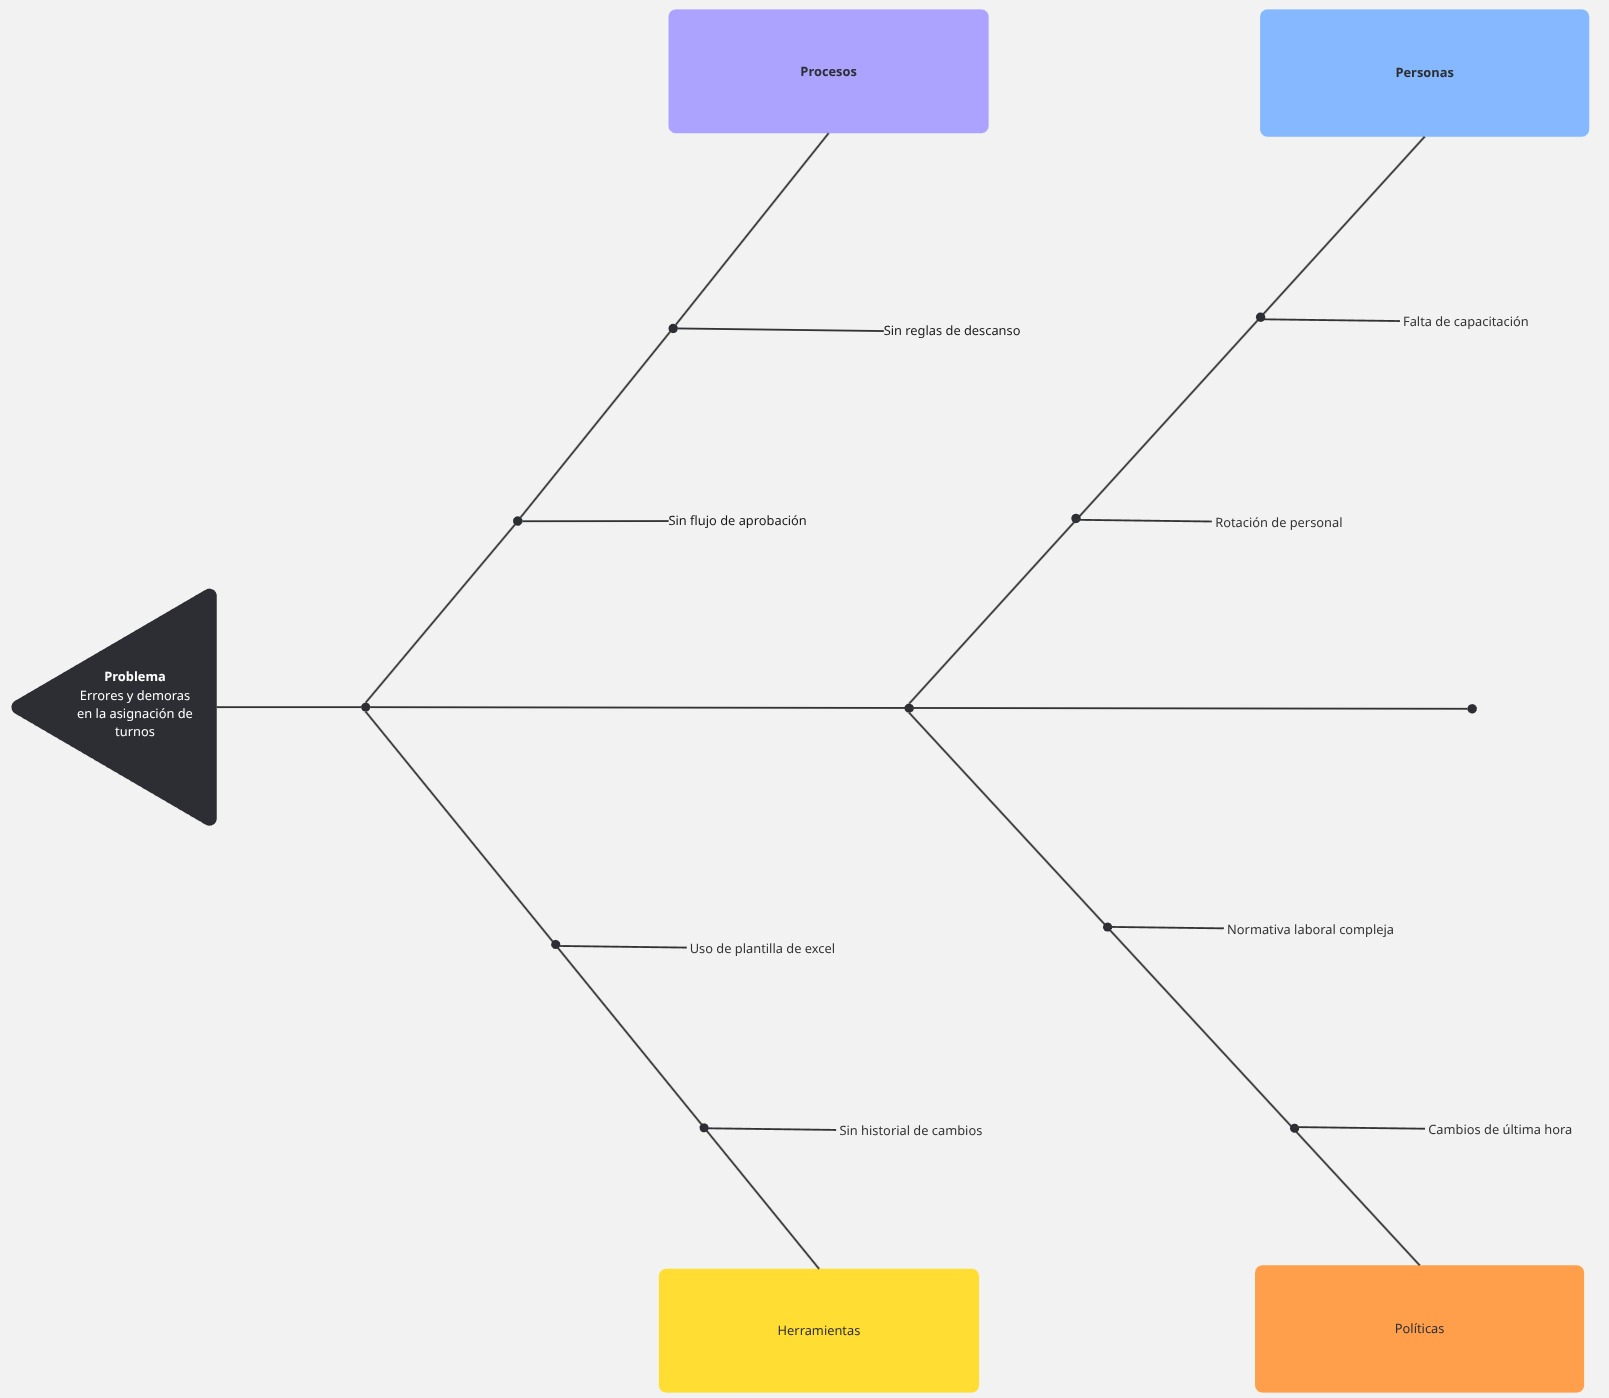
\includegraphics[width=0.9\textwidth]{ishikawa.jpg}
\caption{Diagrama de Ishikawa detallando causas y subcausas del problema.}
\label{fig:ishikawa}
\end{figure}

\noindent Detalle de causas por categoría:

\begin{itemize}[leftmargin=1.2cm]
    \item \textbf{Personas}: alta rotación de personal (disponibilidad que cambia y no se registra) y falta de capacitación del encargado en los procesos de recursos humanos.
    \item \textbf{Proceso}: no existen reglas claras de asignación estandarizadas (descansos mínimos, horas máximas) y no hay un flujo de aprobación formal definido para solicitar cambios.
    \item \textbf{Herramientas}: dependencia de planillas de cálculo o papel, e historial de cambios perdidos por el uso de aplicaciones de mensajería no oficiales (WhatsApp).
    \item \textbf{Políticas}: normativa laboral compleja y cambiante, sumado a licencias médicas o ausencias de última hora que rompen con los lineamientos ya publicados.
\end{itemize}

\end{document}